\documentclass[10pt, aspectratio=169]{beamer}
\usefonttheme{professionalfonts}

\mode<presentation>
{
  \usetheme{Berkeley}
  \usecolortheme{beaver}
  \usefonttheme{default}
  \setbeamertemplate{navigation symbols}{}
  \setbeamertemplate{caption}[numbered]
} 

\setbeamertemplate{footline}{%
  \leavevmode%
  \hbox{%
    \begin{beamercolorbox}[wd=.85\paperwidth,ht=2.5ex,dp=1ex,left]{author in head/foot}%
      \usebeamerfont{author in head/foot}Maxx Seminario, Electronic Circuits, Spring 2026%
    \end{beamercolorbox}%
    \begin{beamercolorbox}[wd=.15\paperwidth,ht=2.5ex,dp=1ex,right]{date in head/foot}%
      \hspace*{0.5em}\insertframenumber{} / \inserttotalframenumber\hspace*{0.5em}%
    \end{beamercolorbox}%
  }%
  \vskip0pt%
}

\usepackage[english]{babel}
\usepackage[utf8x]{inputenc}
\usepackage{tikz}
\usetikzlibrary{shapes.geometric}
\usepackage{pgfplots}
\usepackage{array}
\usepackage{makecell}
\usepackage{verbatim}
\usepackage{graphicx}
\usepackage{subcaption}
\usepackage{amsfonts}
\usepackage{amsmath}
\usepackage{bm}
\usepackage{epstopdf}
\usepackage{circuitikz}
\usepackage{caption}
\usepackage{multirow}
\captionsetup{compatibility=false}
\usepackage[absolute,overlay]{textpos}
\usetikzlibrary{calc}
\usetikzlibrary{pgfplots.fillbetween, backgrounds}
\usetikzlibrary{positioning}
\usetikzlibrary{pgfplots.groupplots}
\usetikzlibrary{plotmarks}
\usetikzlibrary{calc}

\pgfplotsset{compat=1.16}

% Added by Maxx Seminario 01/06/2026 - for colored icons in itemize labels
\usepackage{wasysym} % for smiles and frowns
\newcommand{\neutralface}{%
  \tikz[baseline=-0.6ex]{
    \draw (0,0) circle (0.9ex);
    \fill (-0.35ex,0.25ex) circle (0.12ex);
    \fill ( 0.35ex,0.25ex) circle (0.12ex);
    \draw (-0.35ex,-0.25ex) -- (0.35ex,-0.25ex);
  }%
}

\newcommand{\baditem}{\textcolor{red!70!black}{\frownie}}
\newcommand{\gooditem}{\textcolor{green!60!black}{\smiley}}
\newcommand{\mehitem}{\textcolor{orange!80!black}{\neutralface}}


% =========================
% Solution toggle 
% =========================
\newif\ifshowsolutions
\showsolutionstrue   %  compile WITH solutions
%\showsolutionsfalse %  compile WITHOUT solutions



\title{MOSFET Applications and Frequency Response}
\subtitle{Unit 5: Field-Effect Transistors}
\author{Maxx Seminario}
\institute{University of Nebraska-Lincoln}
\date{Spring 2026}

\begin{document}

\begin{frame}
  \titlepage
\end{frame}

% Slide 2: Lecture Overview
\begin{frame}{Lecture Overview}
\begin{columns}[T]
\begin{column}{0.45\textwidth}
\textbf{Review from Last Lecture}
\begin{itemize}
\item MOSFET small-signal models
\item Transconductance ($g_m$)
\item Output resistance ($r_o$)
\item AC analysis techniques
\end{itemize}
\end{column}

\begin{column}{0.45\textwidth}
\textbf{Learning Objectives}
\begin{itemize}
\item Understand CMOS inverter operation
\item Use inverter as CS amplifier
\item Analyze voltage transfer characteristics
\item Study MOSFET parasitic capacitances
\item Determine frequency response
\end{itemize}
\end{column}
\end{columns}
\end{frame}

% Slide 3: CMOS Inverter Introduction
\begin{frame}{The CMOS Inverter}
\begin{columns}
\begin{column}{0.4\textwidth}
\textbf{Circuit Configuration}

\begin{center}
\begin{circuitikz}[scale=0.8]
% PMOS transistor
\draw (0,4) node[pmos, arrowmos, anchor=D](pmos){};
\draw (pmos.S) -- (0,5.5) node[vdd]{$V_{DD}$};

% NMOS transistor
\draw (0,2) node[nmos, arrowmos, anchor=D](nmos){};
\draw (nmos.S) -- (0,0.5) node[ground]{};

% Connect gates with orthogonal lines
\draw (pmos.G) -- (-1.2,4);
\draw (nmos.G) -- (-1.2,2);
\draw (-1.2,4) -- (-1.2,2);

% Input 
\draw (-1.2,3) -- (-2,3);
\node[ocirc] at (-2,3) {};
\node[left] at (-2,3) {$V_{in}$};

% Output 
\draw (pmos.D) -- (nmos.D);
\draw (0,3) -- (1.5,3);
\node[ocirc] at (1.5,3) {};
\node[right] at (1.5,3) {$V_{out}$};

\end{circuitikz}
\end{center}


\end{column}

\begin{column}{0.6\textwidth}
\textbf{Operating States}

% \vspace{0.3cm}
\begin{table}
\centering
\small
\begin{tabular}{|c|c|c|c|}
\hline
\textbf{$V_{in}$} & \textbf{NMOS} & \textbf{PMOS} & \textbf{$V_{out}$} \\ \hline
Low (0V) & OFF & ON & High ($V_{DD}$) \\ \hline
High ($V_{DD}$) & ON & OFF & Low (0V) \\ \hline
Mid ($V_{DD}/2$) & ON & ON & Transition \\ \hline
\end{tabular}
\end{table}

% \vspace{0.5cm}
\textbf{Key Features:}
\begin{itemize}
\item \gooditem Digital logic: inverts input signal
\item \gooditem Low static power consumption
\item \gooditem Rail-to-rail output swing
\end{itemize}

% \vspace{0.3cm}
\begin{block}{Why CMOS?}
Complementary MOS (CMOS) technology is the dominant logic family because only one transistor conducts in steady state, minimizing power dissipation.
\end{block}
\end{column}
\end{columns}
\end{frame}

% Slide 4: Voltage Transfer Characteristic (VTC)
\begin{frame}{Voltage Transfer Characteristic (VTC)}
\begin{columns}[T]
\begin{column}{0.5\textwidth}
\textbf{VTC Plot: $V_{out}$ vs $V_{in}$}

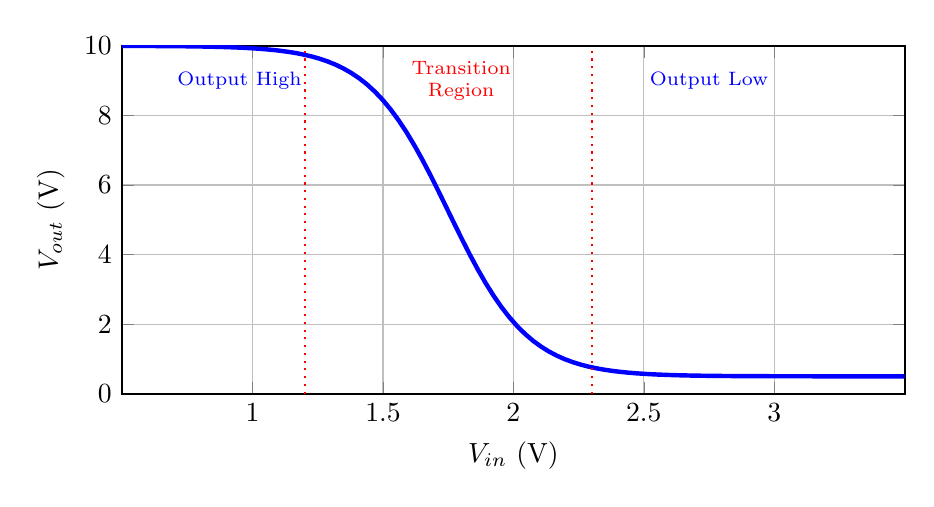
\begin{tikzpicture}
\begin{axis}[
    width=0.95\textwidth,
    height=6cm,
    xlabel={$V_{in}$ (V)},
    ylabel={$V_{out}$ (V)},
    xmin=0.5, xmax=3.5,
    ymin=0, ymax=10,
    xtick={1, 1.5, 2, 2.5, 3},
    ytick={0, 2, 4, 6, 8, 10},
    grid=major,
    thick,
]

% VTC curve
\addplot[blue, ultra thick, domain=0.5:3.5, samples=100] {9.5 / (1 + exp(6.5*(x - 1.75))) + 0.5};

% Vertical dotted lines separating regions
\draw[red, dotted, thick] (axis cs:1.2,0) -- (axis cs:1.2,10);
\draw[red, dotted, thick] (axis cs:2.3,0) -- (axis cs:2.3,10);

% Region annotations
\node[font=\scriptsize, blue] at (axis cs:0.95,9.0) {Output High};
\node[font=\scriptsize, red, align=center] at (axis cs:1.8,9.0) {Transition\\Region};
\node[font=\scriptsize, blue] at (axis cs:2.75,9.0) {Output Low};

\end{axis}
\end{tikzpicture}
\end{column}

\begin{column}{0.5\textwidth}
\textbf{Operating Regions}

\textbf{1. Region I: $V_{in} < V_{th,n}$}
\begin{itemize}
\item NMOS: cutoff
\item PMOS: triode
\item $V_{out} = V_{DD}$
\end{itemize}

\vspace{0.3cm}
\textbf{2. Region II: $V_{th,n} < V_{in} < V_{DD}-|V_{th,p}|$}
\begin{itemize}
\item Both transistors in saturation
\item High gain region (steep slope)
\end{itemize}

\vspace{0.3cm}
\textbf{3. Region III: $V_{in} > V_{DD}-|V_{th,p}|$}
\begin{itemize}
\item NMOS: triode
\item PMOS: cutoff
\item $V_{out} = 0$
\end{itemize}

\end{column}
\end{columns}
\end{frame}

% Slide 5: Inverter as Common Source Amplifier
\begin{frame}{CMOS Inverter as Common Source Amplifier}
\begin{columns}[T]
\begin{column}{0.5\textwidth}
\textbf{Biasing at Transition Point}

\vspace{0.3cm}
\textbf{DC Operating Point:}
\begin{itemize}
\item Set $V_{in,DC} = V_{DD}/2$
\item Both transistors in saturation
\item $V_{out,DC} \approx V_{DD}/2$
\item Maximum small-signal gain
\end{itemize}

\vspace{0.2cm}
\textbf{Voltage Gain:}
\[
A_v = \frac{v_{out}}{v_{in}} = \frac{dV_{out}}{dV_{in}}\bigg|_{Q} < 0
\]

Small input signal produces larger (inverted) output signal


\end{column}




\begin{column}{0.5\textwidth}
\textbf{Small-Signal Operation on VTC}

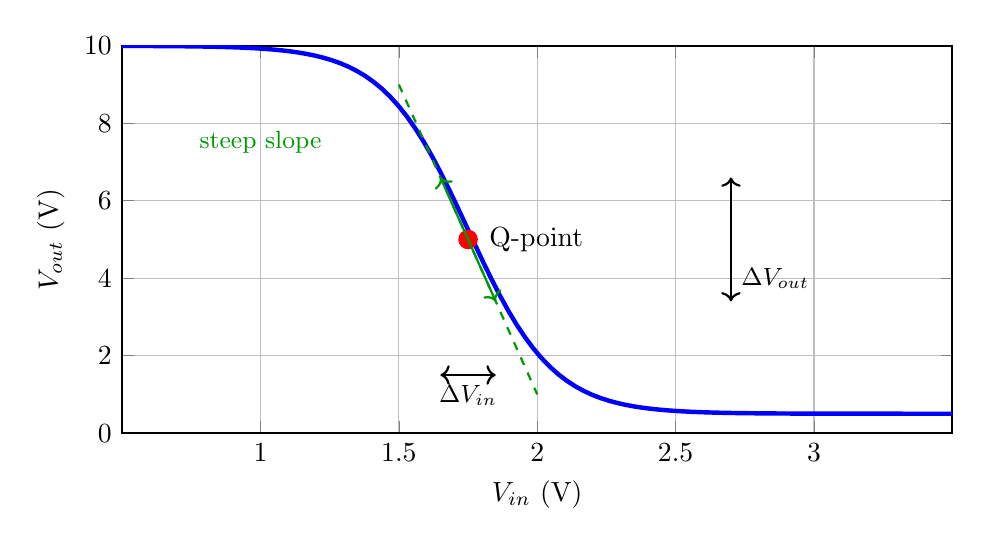
\begin{tikzpicture}
\begin{axis}[
    width=1.0\textwidth,
    height=6.5cm,
    xlabel={$V_{in}$ (V)},
    ylabel={$V_{out}$ (V)},
    xmin=0.5, xmax=3.5,
    ymin=0, ymax=10,
    xtick={1, 1.5, 2, 2.5, 3},
    ytick={0, 2, 4, 6, 8, 10},
    grid=major,
    thick,
]

% VTC curve
\addplot[blue, ultra thick, domain=0.5:3.5, samples=100] {9.5 / (1 + exp(6.5*(x - 1.75))) + 0.5};

% Q-point
\node[circle, fill=red, inner sep=2.5pt, label=right:{Q-point}] at (axis cs:1.75,5) {};

% Small signal variation
\draw[<->, thick, green!60!black] (axis cs:1.65,6.6) -- (axis cs:1.85,3.4);

% Input variation annotation
\draw[<->, thick] (axis cs:1.65,1.5) -- (axis cs:1.85,1.5);
\node[below, font=\small] at (axis cs:1.75,1.5) {$\Delta V_{in}$};

% Output variation annotation
\draw[<->, thick] (axis cs:2.7,3.4) -- (axis cs:2.7,6.6);
\node[right, font=\small] at (axis cs:2.7,4) {$\Delta V_{out}$ };

% Tangent line (slope annotation)
\draw[green!60!black, thick, dashed, domain=1.5:2.0] (axis cs:1.5,9) -- (axis cs:2.0,1);
\node[green!60!black, font=\small] at (axis cs:1,7.5) {steep slope};

\end{axis}
\end{tikzpicture}


\end{column}
\end{columns}
\end{frame}

% % Slide 6: Small-Signal Analysis of CS Amplifier
% \begin{frame}{Small-Signal Analysis of CS Amplifier}
% \begin{columns}[T]
% \begin{column}{0.5\textwidth}
% \textbf{Small-Signal Model}

% \begin{center}
% \begin{circuitikz}[scale=0.8]
% % Input
% \draw (0,2) node[left]{$v_{in}$} to[short, o-] (1,2);

% % Gate to source (open circuit for small signal)
% \draw (1,2) to[short] (2,2);
% \draw (2,0) node[ground]{};

% % Controlled current source
% \draw (2,0) to[american current source, l=$g_m v_{gs}$] (2,4);

% % Output resistance
% \draw (2,4) to[R, l=$r_o$] (4,4);

% % Load resistance RD
% \draw (4,4) to[R, l=$R_D$] (4,0);
% \draw (4,0) node[ground]{};

% % Output
% \draw (4,4) to[short, -o] (5.5,4) node[right]{$v_{out}$};

% % v_gs label
% \node[font=\small] at (1.5,1.8) {$+$};
% \node[font=\small] at (1.5,1) {$v_{gs}$};
% \node[font=\small] at (1.5,0.3) {$-$};

% \end{circuitikz}
% \end{center}

% \vspace{0.2cm}
% \textbf{Key Parameters:}
% \begin{itemize}
% \item $g_m$: transconductance
% \item $r_o$: MOSFET output resistance
% \item $R_D$: drain load resistor
% \item $v_{gs} = v_{in}$ (for AC analysis)
% \end{itemize}
% \end{column}

% \begin{column}{0.5\textwidth}
% \textbf{Gain Derivation}

% At the output node (KCL):
% \[
% g_m v_{gs} + \frac{v_{out}}{r_o} + \frac{v_{out}}{R_D} = 0
% \]

% Since $v_{gs} = v_{in}$:
% \[
% g_m v_{in} + v_{out}\left(\frac{1}{r_o} + \frac{1}{R_D}\right) = 0
% \]

% Solving for voltage gain:
% \[
% A_v = \frac{v_{out}}{v_{in}} = -g_m(r_o \parallel R_D)
% \]

% \[
% \boxed{A_v = -g_m \frac{r_o R_D}{r_o + R_D}}
% \]

% \vspace{0.3cm}
% \textbf{If $r_o \gg R_D$:}
% \[
% A_v \approx -g_m R_D
% \]

% \vspace{0.3cm}
% \textbf{Typical values:}
% \begin{itemize}
% \item $g_m \approx 1-5$ mA/V
% \item $R_D \approx 1-10$ k$\Omega$
% \item $|A_v| \approx 5-20$ (voltage gain)
% \end{itemize}
% \end{column}
% \end{columns}
% \end{frame}

% Slide 7: MOSFET Internal Capacitances
\begin{frame}{MOSFET Internal Capacitances}
\begin{columns}[T]
\begin{column}{0.5\textwidth}
\textbf{Parasitic Capacitances}

\begin{center}
\begin{circuitikz}[scale=0.85, transform shape]
% Bulk ground at top
\draw (1.8,5.5) node[ground, rotate=180]{};
\draw (5.5,5.5) node[ground, rotate=180]{};
\node[above] at (2.0,5.4) {\small B};

% Gate terminal
\draw (0,3.5) node[left]{G} to[short, o-] (1,3.5);

% Gate-to-source capacitance
\draw (1,3.5) to[C, l^=$C_{gs}$] (1,1.5);

% Source terminal
\draw (1,1.5) to[short, -o] (0,1.5) node[left]{S};
\draw (1,1.5) -- (2,1.5);


% Gate-to-drain capacitance
\draw (1,3.5) to[C, l^=$C_{gd}$] (4.6,3.5);

% Drain and source nodes
\draw (4,3.5) -- (5.5,3.5);
\draw (2,1.5) -- (5.5,1.5);

% Controlled current source from drain to source (in parallel with ro)
\draw (3.7,3.5) to[american current source, l=$g_m v_{gs}$] (3.7,1.5);

% Output resistance ro in parallel with current source
\draw (5.5,3.5) to[R, l=$r_o$] (5.5,1.5);

% Drain terminal
\draw (5.5,3.5) to[short, -o] (6.5,3.5) node[right]{D};

% Gate-to-body capacitance (upward to top ground)
\draw (1.8,3.5) to[C, l=$C_{gb}$] (1.8,5.5);

% Drain-to-body capacitance (upward to top ground)
\draw (5.5,3.5) to[C, l=$C_{db}$] (5.5,5.5);

% Source-to-body capacitance (downward to bottom ground)
\draw (1,1.5) to[C, l_=$C_{sb}$] (1,0.5);
\draw (1,0.5) node[ground]{};

% v_gs label
\node[font=\small] at (0.5,3.3) {$+$};
\node[font=\small, align=center] at (0.3,2.5) {$v_{gs}$};
\node[font=\small] at (0.5,1.7) {$-$};

\end{circuitikz}
\end{center}
\end{column}

\begin{column}{0.55\textwidth}
\textbf{1. MOSFET Capacitances}
\begin{itemize}
\item $C_{gs}$: gate-to-source
\item $C_{gd}$: gate-to-drain (feedback path)
\item $C_{gb}$: gate-to-body
\item $C_{db}$: drain-to-body
\item $C_{sb}$: source-to-body
\end{itemize}

% \vspace{0.4cm}
\textbf{Key Points:}
\begin{itemize}
\item In saturation: $C_{gs}$ dominates, $C_{gd}$ and $C_{gb}$ are small
\item $C_{gd}$ creates feedback between input and output
\item Junction capacitances ($C_{db}$, $C_{sb}$) add to load
\end{itemize}

\end{column}
\end{columns}
\end{frame}

% Slide 8: Miller Effect
\begin{frame}{Miller Effect and $C_{gd}$}
\begin{columns}[T]
\begin{column}{0.5\textwidth}
\textbf{The Problem with $C_{gd}$}

\begin{center}
\begin{circuitikz}[scale=0.8, transform shape]
% Gate terminal
\draw (0,3.5) node[left]{G} to[short, o-] (1,3.5);

% Source terminal
\draw (0,1.5) node[left]{S} to[short, o-] (1,1.5);
\draw (1,1.5) -- (2,1.5);

% Gate-to-drain capacitance (feedback path)
\draw (1,3.5) to[C, l^=$C_{gd}$] (4.6,3.5);

% Drain and source nodes
\draw (4,3.5) -- (5.5,3.5);
\draw (2,1.5) -- (5.5,1.5);

% Controlled current source from drain to source (in parallel with ro)
\draw (3.7,3.5) to[american current source, l=$g_m v_{gs}$] (3.7,1.5);

% Output resistance ro in parallel with current source
\draw (5.5,3.5) to[R, l=$r_o$] (5.5,1.5);

% Drain terminal
\draw (5.5,3.5) to[short, -o] (6.5,3.5) node[right]{D};

% Source ground
\draw (1,1.5) to[short] (1,1.3);
\draw (1,1.3) node[ground]{};

% v_gs label
\node[font=\small] at (0.5,3.3) {$+$};
\node[font=\small, align=center] at (0.3,2.5) {$v_{gs}$};
\node[font=\small] at (0.5,1.7) {$-$};

\end{circuitikz}
\end{center}

\vspace{-0.6cm}
\[
i_{gd} = C_{gd}\frac{d(v_{in} - v_{out})}{dt}
\]
\[
i_{gd} = C_{gd}(1 - A_v)\frac{dv_{in}}{dt}
\]

\vspace{-0.3cm}
\textbf{Miller capacitance:}
\[
\boxed{C_{Miller} = C_{gd}(1 - A_v) = C_{gd}(1 + |A_v|)}
\]
\end{column}

\begin{column}{0.5\textwidth}
\textbf{Miller Effect Illustration}

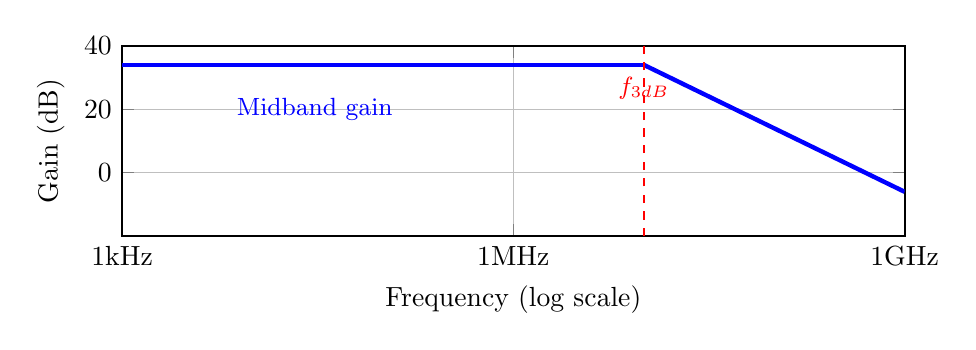
\begin{tikzpicture}
\begin{axis}[
    width=0.95\textwidth,
    height=4cm,
    xlabel={Frequency (log scale)},
    ylabel={Gain (dB)},
    xmode=log,
    xmin=1e3, xmax=1e9,
    ymin=-20, ymax=40,
    xtick={1e3, 1e6, 1e9},
    xticklabels={1kHz, 1MHz, 1GHz},
    ytick={0, 20, 40},
    grid=major,
    thick,
]

% Flat response
\addplot[blue, ultra thick, domain=1e3:1e7] {34};

% Roll-off
\addplot[blue, ultra thick, domain=1e7:1e9] {34 - 20*log10(x/1e7)};

% 3dB point
\draw[red, dashed, thick] (axis cs:1e7,-20) -- (axis cs:1e7,40);
\node[above, red, font=\small] at (axis cs:1e7,20) {$f_{3dB}$};

% Annotations
\node[blue, font=\small] at (axis cs:3e4,20) {Midband gain};
\end{axis}
\end{tikzpicture}

\vspace{-0.2cm}
\textbf{Impact on Bandwidth:}

% Input capacitance:
\[
C_{in} = C_{gs} + C_{gd}(1 + |A_v|)
\]
\[
f_{3dB} = \frac{1}{2\pi R_s C_{in}}
\]

where $R_s$ is the source resistance.

\end{column}
\end{columns}
\end{frame}

% Slide 9: Frequency Response of CS Amplifier
\begin{frame}{Frequency Response of Common Source Amplifier}
\begin{columns}[T]
\begin{column}{0.5\textwidth}
\textbf{Complete High-Frequency Model}
\vspace{-0.1cm}
\begin{center}
\begin{circuitikz}[scale=0.7, transform shape]
% Source
\draw (0,3) to[sV, l=$v_s$] (0,1);
\draw (0,1) node[ground]{};
\draw (0,3) to[R, l=$R_s$] (2,3);

% Input capacitances
\draw (2,3) to[C, l=$C_{gs}$] (2,1);
\draw (2,1) node[ground]{};
\draw (2,3) to[C, l=$C_{gd}$] (4,3);

% Controlled source and output resistance
\draw (4,3) to[american current source, l=$g_m v_{gs}$] (4,1);
\draw (4,1) node[ground]{};
\draw (4,3) to[R, l=$r_o$] (6,3);

% Load
\draw (6,3) to[R, l=$R_L$] (6,1);
\draw (6,1) node[ground]{};
\draw (6,3) to[C, l=$C_L$] (8,3);
\draw (8,3) -- (8,1) node[ground]{};

% Output
\draw (6,3) to[short, -o] (9,3) node[right]{$v_{out}$};

% Label input voltage
\draw (2,3) to[short] (2.5,3);
% \node[above] at (2.5,3.3) {$v_{gs}$};

\end{circuitikz}
\end{center}

\vspace{-0.2cm}
\textbf{Pole Locations:}
\[
\omega_{p1} = \frac{1}{R_s[C_{gs} + C_{gd}(1+g_mR_L)]}
\]
\[
\omega_{p2} = \frac{1}{(r_o \parallel R_L)(C_{gd} + C_L)}
\]
Usually $\omega_{p1} < \omega_{p2}$, so input pole dominates.
\end{column}

\begin{column}{0.5\textwidth}
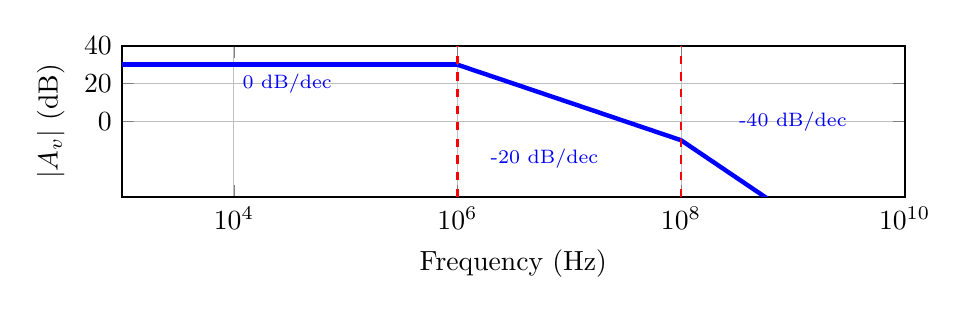
\begin{tikzpicture}
\begin{axis}[
    width=0.95\textwidth,
    height=3.5cm,
    xlabel={Frequency (Hz)},
    ylabel={$|A_v|$ (dB)},
    xmode=log,
    xmin=1e3, xmax=1e10,
    ymin=-40, ymax=40,
    xtick={1e4, 1e6, 1e8, 1e10},
    ytick={0, 20, 40},
    grid=major,
    thick,
]

% Magnitude response
\addplot[blue, ultra thick, domain=1e3:1e6] {30};
\addplot[blue, ultra thick, domain=1e6:1e8] {30 - 20*log10(x/1e6)};
\addplot[blue, ultra thick, domain=1e8:1e10] {30 - 20*log10(1e8/1e6) - 40*log10(x/1e8)};

% Pole markers
\draw[red, dashed] (axis cs:1e6,-40) -- (axis cs:1e6,40);
\node[above, red, font=\small] at (axis cs:1e6,35) {$f_{p1}$};

\draw[red, dashed] (axis cs:1e8,-40) -- (axis cs:1e8,40);
\node[above, red, font=\small] at (axis cs:1e8,35) {$f_{p2}$};

% Slope annotations
\node[blue, font=\scriptsize] at (axis cs:3e4,20) {0 dB/dec};
\node[blue, font=\scriptsize, align=center] at (axis cs:6e6,-20) {-20 dB/dec};
\node[blue, font=\scriptsize, align=center] at (axis cs:1e9,0) {-40 dB/dec};

\end{axis}
\end{tikzpicture}

\vspace{-0.2cm}

\textbf{Design Trade-offs:}
\begin{itemize}
\item Larger $g_m$ $\Rightarrow$ higher gain, lower bandwidth
\item Smaller $R_s$ $\Rightarrow$ higher bandwidth
\item Smaller $W/L$ $\Rightarrow$ lower $C_{gs}$, higher bandwidth
\item Load capacitance $C_L$ limits bandwidth
\end{itemize}
\end{column}
\end{columns}
\end{frame}

% Slide 10: Summary and Design Considerations
\begin{frame}{Summary and Design Considerations}
\begin{columns}[T]
\begin{column}{0.5\textwidth}
\textbf{Key Concepts Covered}

\begin{enumerate}

\item \textbf{Common Source Amplifier}
   \begin{itemize}
   \item Small-signal model: $A_v = -g_m(r_o \parallel R_D)$
   \item Voltage gain proportional to $g_m$
   \item Inverted output signal
   \end{itemize}

\item \textbf{Frequency Limitations}
   \begin{itemize}
   \item Internal capacitances ($C_{gs}$, $C_{gd}$)
   \item Miller effect multiplication
   \item Gain-bandwidth tradeoff
   \end{itemize}


\item \textbf{Practical Applications:}
    \begin{itemize}
    \item Analog amplifiers
    \item Digital logic gates
    \item Mixed-signal circuits
    \item RF amplifiers (with special techniques)
    \end{itemize}

\end{enumerate}
\end{column}


\begin{column}{0.5\textwidth}
\textbf{Design Guidelines}

\vspace{0.3cm}
\textbf{For High Gain:}
\begin{itemize}
\item \gooditem Large $g_m$ (large $W/L$, high $I_D$)
\item \gooditem High $r_o$ (long channel length)
\item \baditem Lower bandwidth (trade-off)
\end{itemize}

\vspace{0.3cm}
\textbf{For High Bandwidth:}
\begin{itemize}
\item \gooditem Small $C_{gs}$ (small $W/L$)
\item \gooditem Minimize $C_{gd}$ (small $L_{ov}$)
\item \gooditem Low source impedance
\item \baditem Lower gain (trade-off)
\end{itemize}


\end{column}
\end{columns}
\end{frame}

% Slide 11: Practice Problem 1
\begin{frame}{Practice Problem 1: CS Amplifier Gain}
\textbf{Problem:}

A common source amplifier has the following parameters:
\begin{itemize}
\item $g_m = 4$ mA/V
\item $r_o = 25$ k$\Omega$
\item $R_D = 2$ k$\Omega$
\end{itemize}

\vspace{0.3cm}
Calculate the small-signal voltage gain.

\ifshowsolutions
\textcolor{blue}{\textbf{Solution:}}

Using the CS amplifier gain formula:
\[
A_v = -g_m(r_o \parallel R_D) = -g_m \frac{r_o R_D}{r_o + R_D}
\]

Substituting the values:
\[
A_v = -4\text{ mA/V} \times \frac{25\text{ k}\Omega \times 2\text{ k}\Omega}{25\text{ k}\Omega + 2\text{ k}\Omega} = -4\text{ mA/V} \times 1.85\text{ k}\Omega = -7.4\text{ V/V}
\]

\textbf{Answer:} $\boxed{A_v = -7.4\text{ V/V}}$
\fi
\end{frame}

% Slide 12: Practice Problem 2
\begin{frame}{Practice Problem 2: Miller Capacitance}
\textbf{Problem:}

For the amplifier in Problem 1, if $C_{gd} = 15$ fF, calculate the Miller capacitance at the input.

\textbf{Given from Problem 1:}
\begin{itemize}
\item $A_v = -7.4$ V/V
\item $C_{gd} = 15$ fF
\end{itemize}

\ifshowsolutions
\textcolor{blue}{\textbf{Solution:}}

The Miller capacitance is given by:
\[
C_{Miller} = C_{gd}(1 - A_v) = C_{gd}(1 + |A_v|)
\]

Substituting the values:
\[
C_{Miller} = 15\text{ fF} \times (1 + 7.4) = 15\text{ fF} \times 8.4 = 126\text{ fF}
\]


\textbf{Answer:} $\boxed{C_{Miller} = 126\text{ fF}}$

\textbf{Note:} The feedback capacitance is multiplied by $(1 + |A_v|)$, increasing it by over 8$\times$. This dramatically reduces the bandwidth.
\fi
\end{frame}


\end{document}
